\section{電源系 (概要/EPS/インヒビット設計(二重絶縁)/電源系統図/電池/SAP)(池谷・中塚)}
\subsection{概要}
本節では本衛星の電源系について述べる.

本衛星の電源系の概要を
に示す.

電源系統図挿入

本衛星の電源系は主に以下のコンポーネントから構成されている.
\begin{itemize}
	\item 太陽電池パネル(Solar Array Panel, SAP)
	\item 電源基板EPS
	\item バッテリ
	\item インヒビット回路
	\item CIB電源系
	\item ミッション部電源系
\end{itemize}


\begin{landscape}
\begin{figure}[htbp]
	\begin{center}
		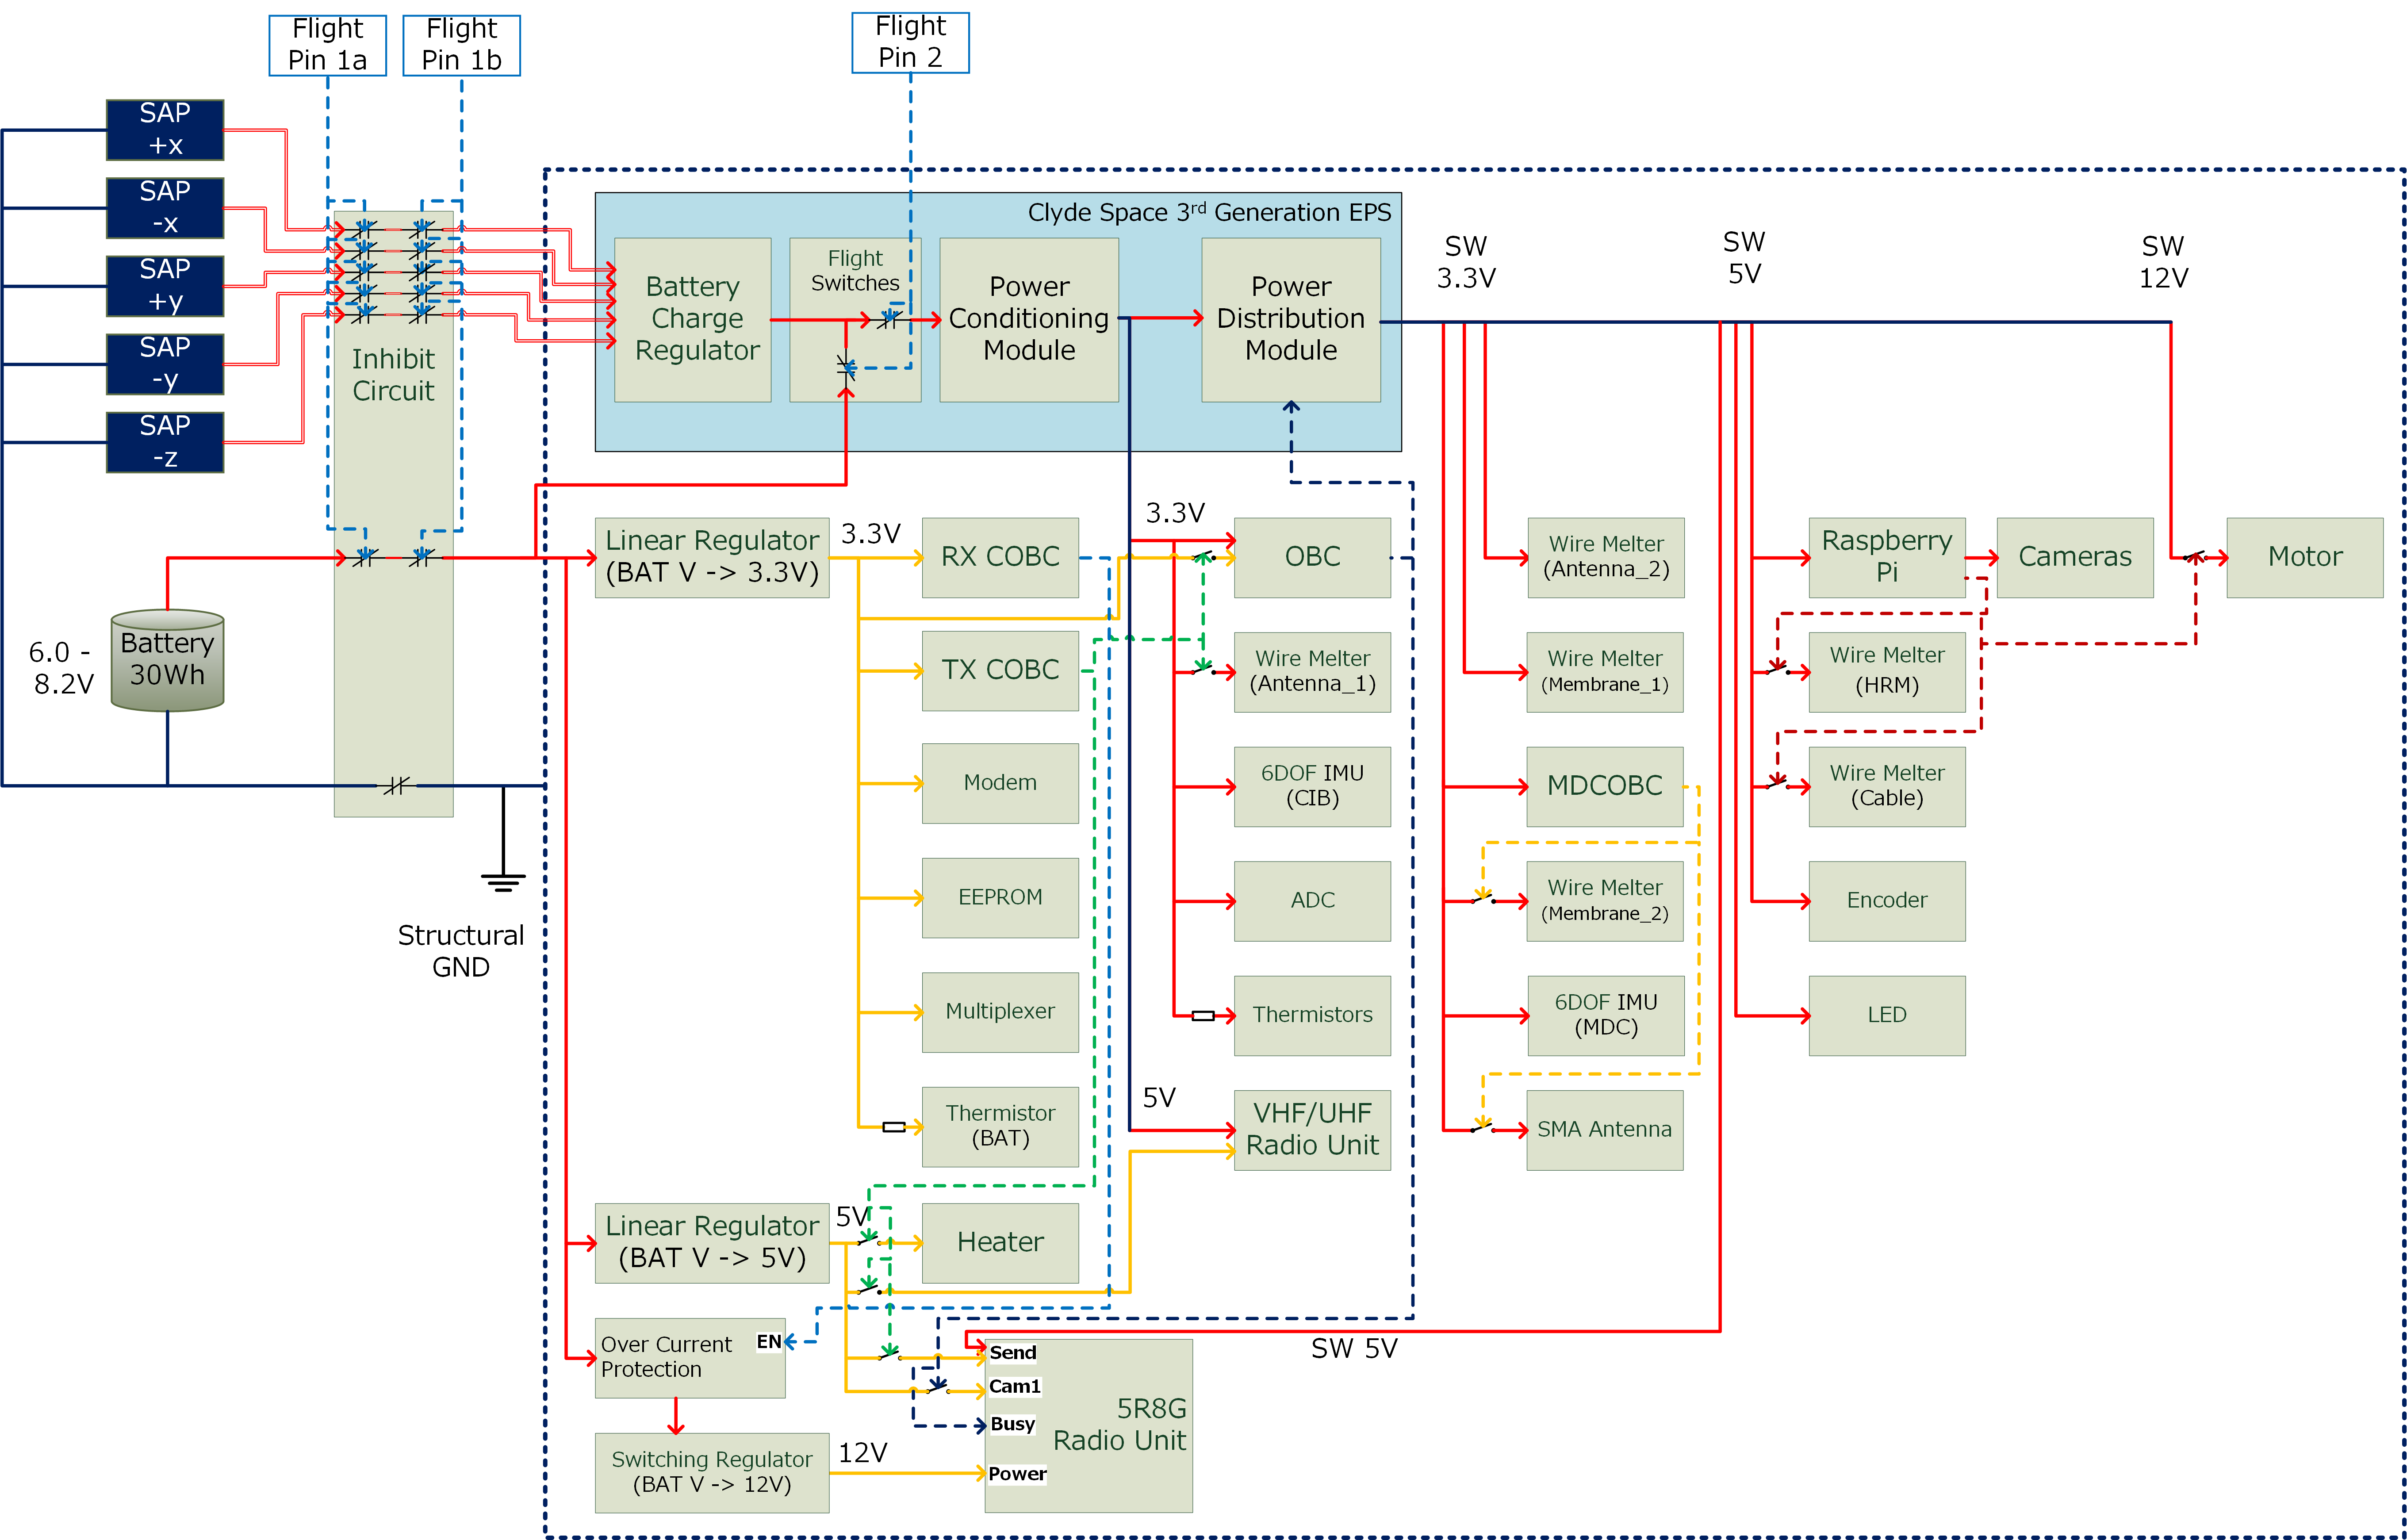
\includegraphics[width=0.5\linewidth]{./03/fig/Power_diagram.png}
		\caption{Example of a figure caption.}
		\label{mir}
	\end{center}
\end{figure}
\end{landscape}            


\subsection{SAP}

\subsubsection{SAP試験}

\subsection{バッテリ}


\subsection{CIB電源系}

\subsection{EPS}


\subsection{ミッション部電源系}